%% Development Process
%%=========================================

\chapter{Development Process}
\label{ch:development_process}
This chapter presents how the development process of our model was conducted. The process is briefly summarized, and is mainly done to illustrate how we used our research methodology to develop our models as a product of working iteratively. Note that this chapter does not present any details about the models architecture, this is done in the next chapter. Also note that because the iteration process not necessarily is followed in a strict manner, iterations that led nowhere are ignored, and some work that was carried out in-between iterations are moved where they fitted best. Some details and work is also omitted, for the sake of having a clear and brief summarizing.

%%=========================================

\section{First Iteration -- Ground Work And Exploration}
The first iteration in the cycle included a lot ground work and some exploration. The work done in this iteration was mostly for exploration to back up claims from the preliminary research phase.

\subsection{Construction Pipeline}
\label{sec:construction_pipeline}




\subsection{First Model Experimentation}
After researching state of the art solutions in the area of machine translation, various sourced had made it very clear that LSTMs alone could not handle a sequence to sequence problem. \citep{sutskever2014sequence} stated in the description of their purposed model:

\begin{quote}
    The RNN can easily map sequences to sequences whenever the alignment between the inputs the outputs is known ahead of time. However, it is not clear how to apply an RNN to problems whose input and the output sequences have different lengths with complicated and non-monotonic relationships.
\end{quote}

In our particular problem, this alignment is not know, and this makes it difficult for our model to map input to output in a sensible way. One input of our problem does not necessarily map directly to an output. This creates an alignment difference between input and output where the input in most cases will be much wider than the output. This is exactly the problem pointed out by \citep{sutskever2014sequence}.

\begin{figure}[H]
    \centering
    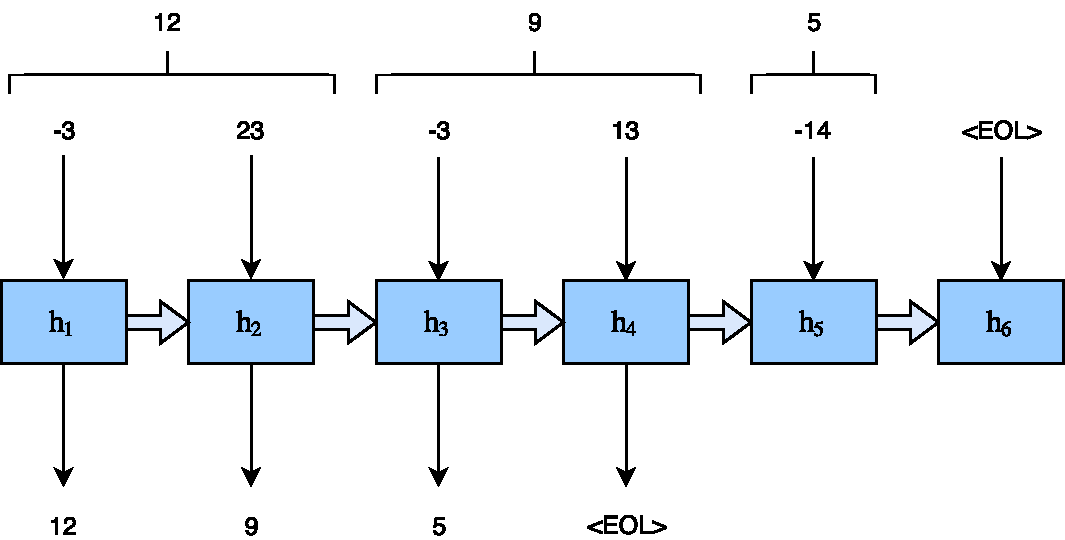
\includegraphics[width=1\textwidth]{fig/development_process/lstm-alignment.pdf}
    \caption{Alignment between input and output in a recurrent neural network}
    \label{fig:lstm-alignment}
\end{figure}

Figure \ref{fig:lstm-alignment} illustrates the difference in the alignment between input and output, reusing the data from Table \ref{eq:input_stop_words} without stop words. The alignment difference means that the first output of the model depends on the input it has yet to see, which the model can not know. The difficulties with the alignment made projecting output through a LSTM using its hidden state would be meaningless. 

Testing a LSTM model that simply projected its hidden states to the output gave very poor results. It was clear, both from theory and from results, that such an approach would not be suitable for our problem. We already knew that the encoder-decoder architecture did not have this problem, and we noted for the next iteration how to proceed with the development of our model. 

%%=========================================

\section{Second Iteration -- Projecting Vector}
The first iteration made it clear that simply projecting hidden states of LSTMs was not suitable for our problem. The second iteration used an approach that repeats a vector across time steps. This approach is architecturally not very different from an encoder-decoder, but lacks some of the characteristics that characterizes an encoder-decoder model.

This model, called {\tt RepVec}, short for ``repeat vector", can be seen as a ``poor man's encoder-decoder", as we will see in section yy. We decided to implement this model as it was sort of a middle ground between the LSTM approach from the previous iteration, and a complete encoder-decoder model. Implementing this solution was mostly done to see if we could solve the problem without investing in a complex system that relied on the encoder-decoder. Weather or not the model was successful, it would tell us how LSTMs could work with our problem if we removed the alignment complications from the equation.

%%=========================================

\section{Third Iteration -- Encoder-Decoders}
With the first model developed during the previous iteration, this iteration focused on developing fully fleshed out encoder-decoder models. We knew this would could likely be the best performing model based on the studies conducted earlier. All research pointed in the direction of an encoder-decoder model for a problem similar to ours. The main reason we had not skipped directly to testing one of these out what for the sake of the ``design and creation" and its iteratively approach to solving problems, as well as taking our time to explore possibilities. The earlier iterations had also given us valuable insights in the nature of our problem.

There were developed two separate models in this iteration. These were encoder-decoders with and without attention. These were named {\tt EncDecReg} and {\tt EncDecAtt} respectively, short for ``encoder-decoder regular" and ``encoder-decoder attention".

%%=========================================

\section{Fourth Iteration -- Parameter Adjustments}
The previous iteration saw the implementation of the two encoder-decoder models. We had also implemented a model based on repeating LSTM output before that. Some minor testing of these models had been carried up until this point, but this iteration was mostly dedicated to tuning the models for better performance. This was done by running bigger test and and exploring various configurations in ways we felt made sense. 

Despite the time we spent on these adjustments, there are bound to be ways to get the models to behave even better. The configurations we ended up with were not that different from the default options in the frameworks we used, and a lot time was spent to understand why things were configured like it was, not necessarily changing it completely. Our models also archived relatively good results on the tests we ran, so we saw no reason to dismantle the models completely to gain an insignificant improvement.

%%=========================================

\section{Fifth Iteration -- Finalization and Cleanup}
The fifth, and final iteration, saw the finalization of system. This included reimplementing some parts of the system that over the course of the development grew far too complex. While this did not benefit us directly as the work on the system was already completed, we wanted the system to be tidy and the code to following the coding standards.